\documentclass[xcolor=pdftex,dvipsnames,table]{beamer}
\usepackage{xcolor}
\usepackage{beamerthemeshadow}
\usepackage{verbatim}
\usepackage{lastpage}
\usepackage{pgf}
\usepackage{colortbl}
\usepackage{hyperref}
\usepackage{multirow}
\usepackage{dsfont}
\usepackage{graphbox}
\usepackage[brazilian]{babel}
\usepackage[utf8]{inputenc}
\usepackage[T1]{fontenc}
\usepackage{tikz}
\usepackage[alf]{abntex2cite}


%----------------------------------------------------
\usepackage{ragged2e}
\usepackage{listings}
\usepackage{multicol} 
\setlength{\columnsep}{1cm}

\lstset{ 
  language=c,                    % the language of the code
  keywordstyle=\color{Black},         % keyword style
  commentstyle=\color{ForestGreen},   % comment style
  stringstyle=\color{RoyalBlue},      % string literal style
  columns=fullflexible,
   literate=%
         {á}{{\'a}}1
         {í}{{\'i}}1
         {é}{{\'e}}1
         {ú}{{\'u}}1
         {ó}{{\'o}}1
         {Á}{{\'A}}1
         {Í}{{\'I}}1
         {É}{{\'E}}1
         {Ý}{{\'Y}}1
         {Ú}{{\'U}}1
         {Ó}{{\'O}}1
         {ã}{{\~a}}1   
         {õ}{{\~o}}1
         {ç}{{\c{c}}}1
         {Ã}{{\~A}}1
         {Õ}{{\~O}}1
         {Ç}{{\c{C}}}1  
         {à}{{\`a}}1
         {â}{{\^a}}1      % acentos
} 

\addtobeamertemplate{navigation symbols}{}{%
    \usebeamerfont{footline}%
    \usebeamercolor[fg]{footline}%
    \hspace{1em}%
    \insertframenumber/\inserttotalframenumber
}
%----------------------------------------------------

\usepackage{siunitx}
\sisetup{input-symbols=(), group-digits  = false} 

\definecolor{light}{rgb}{1.0,0.7,0.7}
\definecolor{BrickRed}{rgb}{0.8,0.1,0.1}
\definecolor{light}{rgb}{1.0,0.5,0.5}
\newcommand{\hl}[1]{\only<#1>{\cellcolor{light}}}

\definecolor{mycolor}{rgb}{0.25,0.0,0.37}
\usecolortheme[named=mycolor]{structure}


\hypersetup{colorlinks,
citecolor=blue,
linkcolor=.,
menucolor=white,
filecolor=blue,   
anchorcolor=yellow
}


\newcommand{\ft}{\frametitle}

\title[Dynare]{Introdução ao Dynare} \subtitle{Modelos dinâmicos e estocástico de equilíbrio geral}
\author[Alves, C. A.]
{
Cássio Roberto de Andrade Alves\\
PPGEco/UFSC \\
Orientador: Prof. Dr. Guilherme Valle Moura
}
\date{\today}


\begin{document}

\frame[plain]{\titlepage \setcounter{framenumber}{0}}

%=============================================================
\section{Introdução}
%=============================================================

\begin{frame}
\ft{Introdução}

Tópicos abordados:

\begin{enumerate}
\item Explicação sobre o Dynare.
\item Resolver modelo de expectativas racionais.
\item Gerar Função impulso-resposta do Modelo Novo Keynesiano básico.
\item Simular séries.
\end{enumerate}

\end{frame}

%----------------------------------------------------------------

\begin{frame}
\ft{Introdução}
\framesubtitle{O que é o Dynare}

	\begin{itemize}
	\item É um software para trabalhar com uma ampla gama de modelos econômicos;
	
	\item É `executado' no Matlab ou octave;
	
	\item Permite trabalhar com modelos determinísticos e estocásticos;

	\item Vamos focar nos modelos estocásticos (D\textbf{S}GE).
	\end{itemize}

\end{frame}

%-----------------------------------------------------------------
\begin{frame}
\ft{Introdução}
\framesubtitle{O que o Dynare pode fazer?}
\begin{itemize}

\item O Dynare permite trabalhar com modelos calibrados.
	
	\begin{itemize}
	\item Encontrar as funções políticas;
	
	\item Simular as séries de tempo;
	
	\item Análise de impulso-resposta.
	\end{itemize}
\pause
\item E permite também trabalhar com estimação de modelos de expectativas racionais (ER).

	\begin{itemize}
	\item Estimação Clássica;
	\item \textbf{Estimação Bayesiana}.
	\end{itemize}

\end{itemize}
\end{frame}

%--------------------------------------------------------------------------------

\begin{frame}[fragile]
\ft{Como o Dynare funciona?}

\begin{figure}[h!]
\includegraphics[scale=0.35]{fig0.png}
\label{fig1}
\end{figure}

\end{frame}

%--------------------------------------------------------------------------------

%=============================================================
\section{Modelo}
%=============================================================

\begin{frame}
\ft{Modelo Novo-Keynesiano}

\begin{itemize}
\item Como exemplo de modelo de ER, considere o modelo Novo-Keynesiano básico.

\item O Dynare \textit{aceita} tanto modelo não-linear quanto modelo log-linear(izado).

\begin{block}{Exemplo utilizado}
Considere o modelo Novo-Keynesiano log-linearizado.
\end{block} 

\end{itemize}
\end{frame}

%-------------------------------------------------------------------------------
\subsection{Equações microfundamentadas}
\begin{frame}[fragile]
\ft{Modelo}
\begin{itemize}
\item O modelo pode ser resumido com as seguintes equações:
\vspace{-0.4cm}
\begin{align}
\pi_t &= \beta \mathbb{E}_t[\pi_{t+1}] + \kappa	\tilde{y}_t
\label{eq1} \\
\tilde{y}_t &= \mathbb{E}_t[\tilde{y}_{t+1}] - \frac{1}{\sigma}\left(R_t - \mathbb{E}_t[\pi_{t+1}] - r_t^n \right) 
\label{eq2} \\
i_t &= \phi_{\pi} \pi_t +\phi_y \tilde{y}_t + \nu_t
\label{eq3}\\
r_t^n &= \sigma \psi_n^{ya}(\mathbb{E}_t[a_{t+1}] - a_t)
\label{eq4}\\
r_t &= i_t - \mathbb{E}_t[\pi_{t+1}]
\label{eq5}\\
y_t^n &= \psi_{ya}^n a_t
\label{eq6}\\
\tilde{y}_t &= y_t - y_t^n
\label{eq7}\\
m_t &= y_t - \eta i_t
\label{eq8}\\
y_t &= a_t +(1-\alpha)n_t
\label{eq9}
\end{align}

\end{itemize}
\end{frame}

%--------------------------------------------------------------------------------
\subsection{Choques exógenos e v. anuais}

\begin{frame}[fragile]
\ft{Modelo (continuação...)}

\begin{itemize}
\item As figuras reportadas por \citeonline{gali2008} mostram algumas variáveis anualizadas. Além dos processos AR, acrescentei as seguintes eq.:
\end{itemize}
\vspace{-0.4cm}
\begin{align}
\nu_t &= \rho_{\nu} \nu_{t-1} + \epsilon_t^{\nu}
\label{eq10}\\
a_t &= \rho_a a_{t-1} + \epsilon_t^a
\label{eq11}\\
i_t^{(anual)} &= 4 i_t
\label{eq12}\\
r_t^{(anual)} &= 4 r_t
\label{eq13}\\
r_t^{n(anual)} &= 4 r_t^n
\label{eq14}\\
\pi_t^{(anual)} &= 4 \pi_t
\label{eq15}\\
\Delta m_t^{(anual)} &= 4[(y_t - y_{t-1}) - \eta (i_t - i_{t-1}) + \pi_t]
\label{eq16} 
\end{align}

\end{frame}


%--------------------------------------------------------------------------------

\begin{frame}[fragile]
\ft{Modelo (continuação...)}

\begin{itemize}
\item No Dynare escrevemos as equações da forma como está em (\ref{eq1})-(\ref{eq16})
\item Mas é importante saber que esse modelo pode ser escrito na forma matricial, coletando todas as variáveis em um vetor $X_t$:

\begin{align}
\Gamma_0 X_t = \Gamma_1 X_t + \Psi \epsilon_t + \Pi \eta_t
\label{eq17}
\end{align}

\item E então um método pode ser utilizado para resolver o modelo. Os métodos mais utilizados:

	\begin{itemize}
	\item \citeonline{blanchard1980}
	\item \citeonline{sims2002}
	\item \citeonline{klein2000}
	\end{itemize}
\footnotesize{Para uma exposição desses métodos ver \citeonline{dejong2011}}
\end{itemize}

\end{frame}
%--------------------------------------------------------------------------------

\begin{frame}[fragile]
\ft{Modelo}
\begin{itemize}

\item A solução do modelo na forma canônica de (\ref{eq17}) pode ser escrita por:

\begin{align}
X_t = \Phi X_{t-1} + R \epsilon_t
\end{align}

\item Assim, tem-se as funções políticas e se pode fazer a análise de impulso-resposta

\footnotesize{Sobre o método utilizado pelo Dynare ver \citeonline{villemot2011}}

\end{itemize}
\end{frame}

\section{Dynare}
%--------------------------------------------------------------------------------
\begin{frame}[fragile]
\ft{Primeiros passos no código}

\begin{itemize}
\item Podemos dividir nosso código em quatro seções.
\end{itemize}

\begin{block}{Estrutura}
\begin{lstlisting}
// Preâmbulo

// Modelo

// Choques

// Simulação/Estimação
\end{lstlisting}
\end{block}

\end{frame}

%--------------------------------------------------------------------------------

\begin{frame}
\ft{Boas práticas no Dynare}

\begin{enumerate}
\item No Dynare, sempre finalizamos uma linha de código com ponto-vírugla `;'

\item Devemos tomar cuidado com o nome de algumas variáveis ou parâmetros:

	\begin{itemize}
	\item Por exemplo, `alpha', `beta', etc. são nomes reservados do Dynare/Matlab.
	
	\item Por conta disso, devemos evitá-los.
	
	\item Sugestão: 
	
	alpha $\longrightarrow$ alppha
	
	beta  $\longrightarrow$ betta
	
	\end{itemize}

\end{enumerate}
\end{frame}

%----------------------------------------------------------------------------------

\begin{frame}[fragile]
\ft{Boas práticas no Dynare}

\begin{enumerate}
\item Lembrar de fechar os blocos com \textbf{end;}.

\item Convenção temporal.

\begin{itemize}
\item No Dynare o período de uma variável se refere ao momento em que a variável é decidida.

\item Para denotar o tempo usamos:

$y_t$  $\longrightarrow$  y

$\mathbb{E}_t[y_{t+1}]$ $\longrightarrow$ y(+1)

$y_{t-1}$  $\longrightarrow$ y(-1)


\begin{block}{Modelos com Variáveis predeterminadas}

\begin{itemize}
\item É comum alguns artigos apresentarem a lei de movimento de algumas variáveis predeterminadas com a notação em $t+1$.

\item Por exemplo, modelos que incluem uma lei de movimento para o capital $k_t$.

\item No entanto, no Dynare essas variáveis entram como período $t$.
\end{itemize}
\end{block}

\end{itemize}
\end{enumerate}

\end{frame}

%----------------------------------------------------------------------------------

\subsection{Preâmbulo}

\begin{frame}[fragile]
%\ft{Dynare}

\begin{block}{1. Preâmbulo}

	\begin{lstlisting}
// Variáveis do Modelo
var ppi y_gap i r_nat r_real y_nat nu ... m_real;     
		
// Variáveis exógenas
varexo eps_nu eps_a;

// Parâmetros
parameters betta siggma phi epsilon phi_pi phi_y ... eta;

// Valores dos parâmetros
betta  = 0.99;
siggma = 1;
...
eta    = 6;
	
	\end{lstlisting}

\end{block}

\end{frame}

%-----------------------------------------------------------------------------------

\subsection{Modelo (CPO's)}

\begin{frame}[fragile]
\begin{block}{2. Modelo}
	\begin{lstlisting}
model(linear);
	// Parâmetros compostos
	#Omega    = (1-alppha)/(1-alppha+alppha*epsilon);
	...
	#kappa    = lambda*(siggma+(phi+alppha)/(1-alppha));
	
	// Equações
	// 1. Curva de Phillips Novo-Keynesiano
	ppi = betta*ppi(+1) + kappa*y_gap;
	...
	// 16. Demanda real por moeda
	m_real = y-eta*i;
end;
	
	\end{lstlisting}

\end{block}
\end{frame}
%-----------------------------------------------------------------------------------

\subsection{Choques}

\begin{frame}[fragile]
\begin{block}{3. Choques}
	\begin{lstlisting}
shocks;
	var eps_nu = 0.25^2; 
	var eps_a  = 1^2; 
end;	
	\end{lstlisting}
\end{block}

\end{frame}
%-----------------------------------------------------------------------------------

\subsection{Solução do modelo}

\begin{frame}[fragile]

\begin{block}{4. Simulação}
	\begin{lstlisting}
// Estado estacionário: todos iguais a zero nesse caso

resid(1);
steady;
check;

// Simulação e FIR

stoch_simul(order = 1, irf=12, periods=200)
y_gap pi_an y n i_an r_real_an m_cresc_an a;

// Existem outras opções de parâmetros para stoch_simul
// Ver na documentação	
	\end{lstlisting}
\end{block}

\end{frame}

%----------------------------------------------------------------------------------

\begin{frame}[fragile]
\ft{Executando o código no Matlab}

\begin{itemize}
\item Quando terminamos o código no arquivo .mod, rodamos ele no Matlab

\item Antes, porém, precisamos adicionar o caminho do Dynare.

\item Isso pode ser feito por meio do botão ``set path'' -> ``add folder''...

\item Ou pela linha de comando (Windows):

\begin{lstlisting}
>> addpath c:\dynare\4.x.y\matlab
\end{lstlisting}

\item Ajuste x e y para versão do Dynare que você instalou

\item Caso tenha instalado em uma pasta diferente da padrão, ajuste o caminho.
\end{itemize}

\end{frame}

%----------------------------------------------------------------------------------

\begin{frame}[fragile]
\ft{Executando o código no Matlab}

\begin{itemize}
\item Ou pela linha de comando (Linux):

\begin{lstlisting}
>> addpath /usr/lib/dynare/matlab
\end{lstlisting}

\item Além disso, o diretório corrente do Matlab deve estar na pasta que contem o .mod

\item Com os requisitos acima satisfeitos, basta chamar o arquivo .mod por:


\begin{lstlisting}
>> dynare NOME_DO_ARQUIVO.mod
\end{lstlisting}


\end{itemize}
\end{frame}


%----------------------------------------------------------------------------------
\begin{frame}
\ft{Função impulso-resposta: choque de política monetária}

\begin{figure}[h!]
\includegraphics[scale=0.35]{fig31.eps}
\label{fig1}
\end{figure}


\end{frame}
%-----------------------------------------------------------------------------------

\begin{frame}
\ft{Função impulso-resposta: choque em tecnológico}

\begin{figure}[h!]
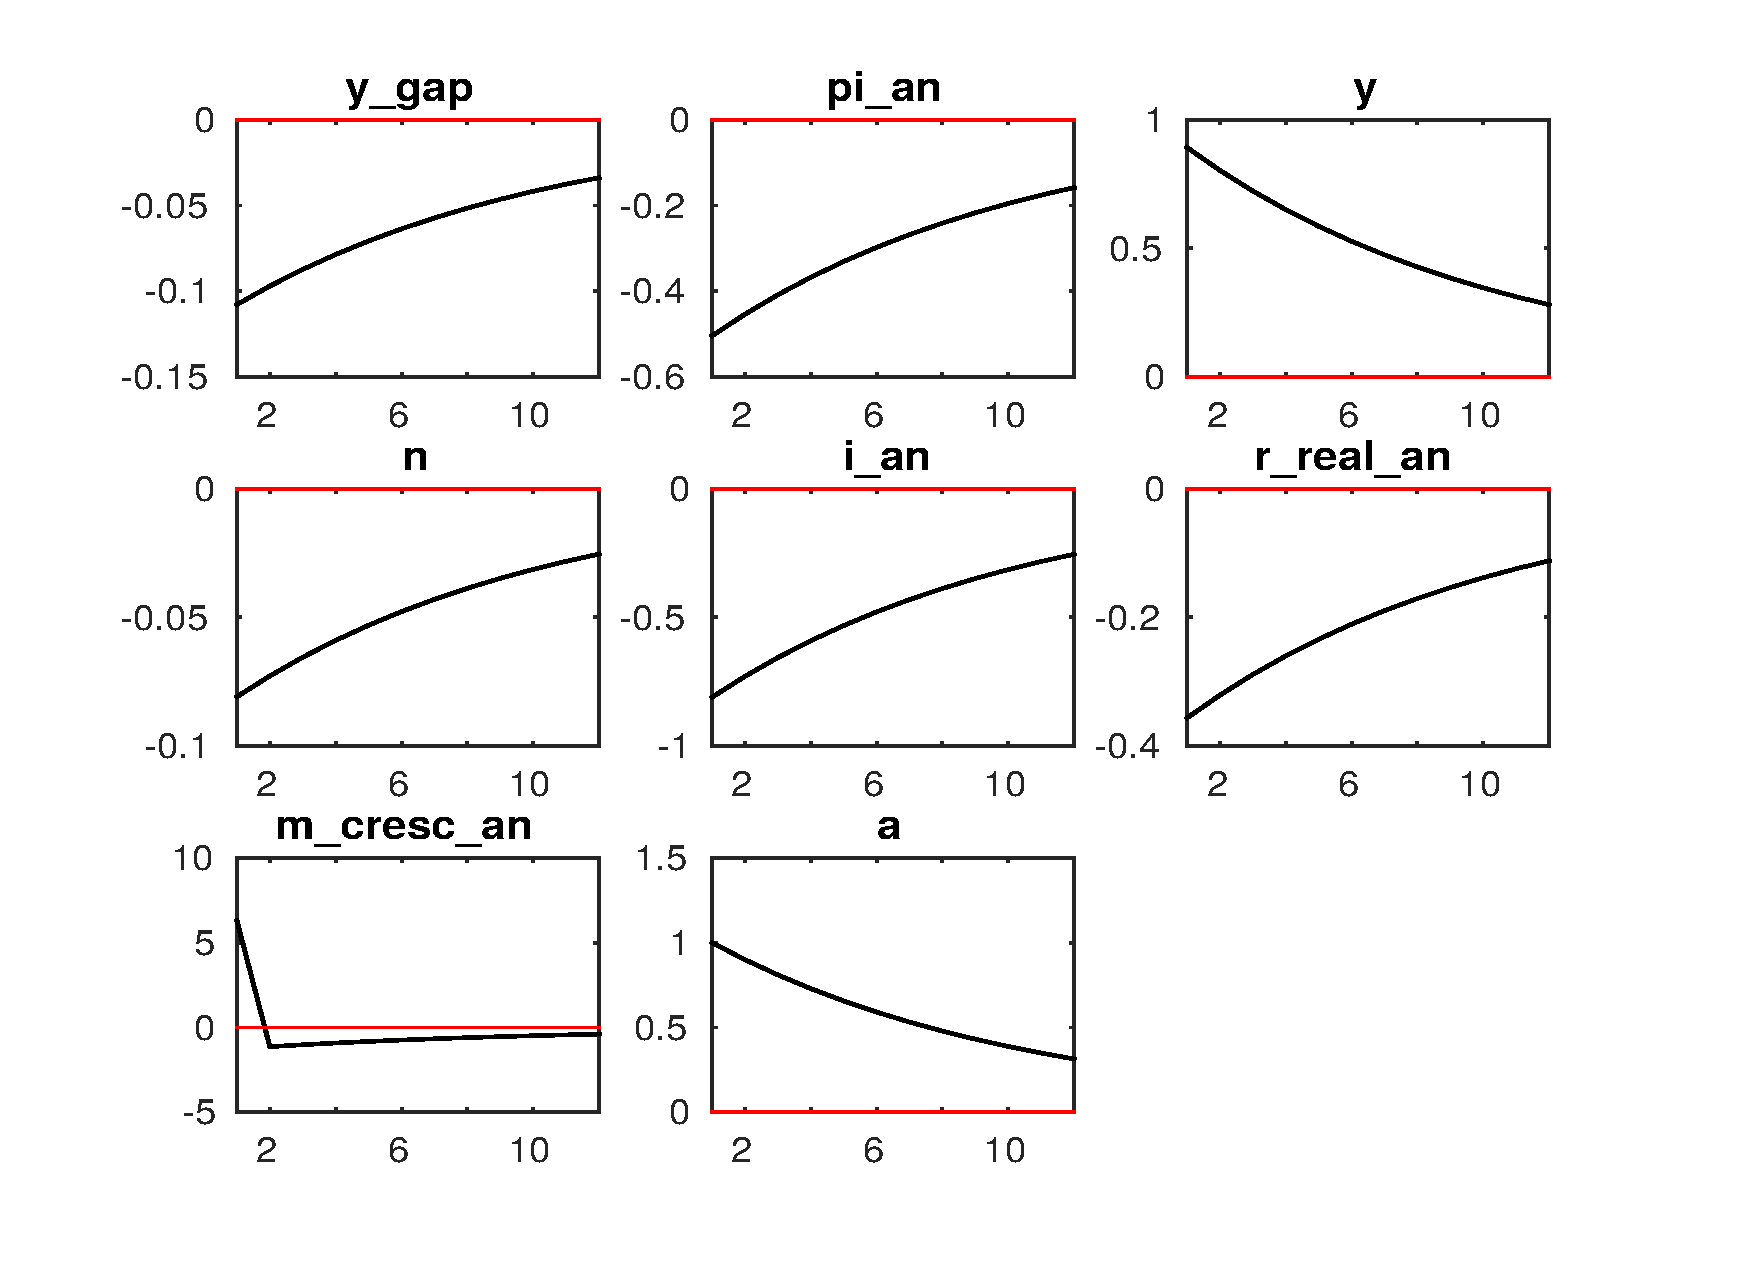
\includegraphics[scale=0.35]{fig32.eps}
\label{fig1}
\end{figure}

\end{frame}

%-----------------------------------------------------------------------------------

\begin{frame}[fragile]
\ft{Interpretação dos resultados}

\begin{itemize}

\item Além das FIR geradas pelo comando stoch\_sim, o Dynare imprime outros resultados na tela.

\item (Ver no Matlab os principais resultados)

\end{itemize}

\begin{enumerate}

\item Autovalores e condição de \citeonline{blanchard1980}.

\item Resumo do modelo.

\item Matriz de covariância dos choques exógenos.

\item Funções políticas.

\end{enumerate}
\end{frame}

%------------------------------------------------------------------------------------

\begin{frame}[fragile]
\ft{Onde os resultados foram armazenados?}

\begin{itemize}
\item Em geral, as rotinas de Matlab criada pelo Dynare se encarrega de criar uma pasta no diretório e salvar alguns resultados

\item As figuras geradas, por exemplo, são automaticamente salvas.

\item A pasta $oo\_$ armazena os resultados

\item E podemos acessá-los via linha de comando

\item Por exemplo:

\begin{lstlisting}
>> oo_.irfs
\end{lstlisting}

para acessar as funções impulso resposta.
\item Com isso, uma das possibilidades é usar as ferramentas do Matlab para trabalhar com nossos resultados.
\end{itemize}

\end{frame}

%-------------------------------------------------------------------------------------

\begin{frame}[fragile]
\ft{Resultados}

\begin{itemize}
\item Podemos acessar, por exemplo, a série gerada para o hiato do produto:

\begin{lstlisting}
>> oo_.endo_simul(1,:)
\end{lstlisting}

\item Bem como plotar um gráfico como é usual no Matlab

\begin{lstlisting}
>> plot(oo_.endo_simul(1,:))
\end{lstlisting}

\item Essa é uma forma de customizar nossos gráficos e não usar o padrão o Dyanre.

\end{itemize}

\end{frame}

%-------------------------------------------------------------------------------------

\begin{frame}
\begin{figure}[h!]
\includegraphics[scale=0.35]{hiato.pdf}
\label{fig1}
\end{figure}
\end{frame}

%-------------------------------------------------------------------------------------

\section{Estimação}

\begin{frame}
\ft{Estimação de parâmetros}

\begin{itemize}
\item Até aqui tratamos os parâmetros como conhecidos, i.e, calibramos o modelo.

\item Podemos também estimar esses parâmetros.

\item A abordagem bayesiana possui algumas vantagens por permitir incorporar informações de estudos anteriores.

\item Além disso, o uso de distribuições a priori estabiliza a estimação dos
parâmetros, o que é importante especialmente em contexto de séries
de tempo curtas.
\end{itemize}
\end{frame}
%-------------------------------------------------------------------------------------

\begin{frame}
\ft{Estimação de parâmetros}

\begin{itemize}
\item O arquivo .mod para estimação de parâmetros é parecida com o modelo calibrado

\begin{block}{Dica}
Quando vamos estimar um modelo é interessante fazer uma versão calibrada com parâmetros ``razoáveis''. Isso pode nos ajudar a identificar algum possível erro no .mod.
\end{block}

\item Até o bloco que computa o estado estacionário, o código é exatamente o mesmo do modelo calibrado.

\item O próximo passo é declarar as variáveis observáveis.
\end{itemize}
\end{frame}
%-------------------------------------------------------------------------------------


\begin{frame}[fragile]
\ft{Estimação de parâmetros}

\begin{itemize}
\item Observações:

	\begin{enumerate}
	\item As variáveis observáveis devem manter uma simetria com o modelo teórico.
	\item Caso a variável observável não seja exatamente simétrica com o modelo teórico, por exemplo, $\tilde{y}_t^{obs}=\tilde{y}_t$, será necessário incluir as equações de medida.
	
	\footnotesize{A esse respeito ver \citeonline{pfeifer2014} }
	
	\item É necessário que o número de observáveis seja menor ou igual ao número de choques.
	\end{enumerate}
\end{itemize}

\begin{block}{Declarando variáveis observáveis}
\begin{lstlisting}
// Variáveis observáveis
varobs ppi i;
\end{lstlisting}
\end{block}

\end{frame}

%-----------------------------------------------------------------------------------

%\begin{frame}[fragile]
%\ft{Estimação}
%
%\begin{itemize}
%\item 
%\end{itemize}
%
%\end{frame}


\begin{frame}[fragile]
%\ft{Estimação de parâmetros}
%\framesubtitle{}

\begin{block}{Parâmetros estimados e distribuição a priori}
\begin{lstlisting}
estimated_params;
/* PARAM NAME, INITVAL, LB, UB, 
   PRIOR_SHAPE, PRIOR_P1, PRIOR_P2 */
phi_pi, , , ,  normal_pdf, 1.5, 0.05;
phi_y, , , ,  gamma_pdf, 0.25, 0.1;
betta, , , ,  beta_pdf, 0.5, 0.25;
rho_nu, , , ,  beta_pdf, 0.5, 0.25;
rho_a, , , , beta_pdf, 0.5, 0.25;

stderr eps_nu,  inv_gamma_pdf, 0.5, inf; // dp do choque nu
stderr eps_a,  inv_gamma_pdf, 0.5, inf;  // dp do choque a
end;
\end{lstlisting}

\end{block}

\end{frame}

%-------------------------------------------------------------------------------

\begin{frame}[fragile]
\ft{Estimação de parâmetros}

\begin{itemize}
\item Podemos passar os valores iniciais usando o seguinte comando:


\begin{block}{Valores iniciais para max. a posteriori}
\begin{lstlisting}
/* Usa os valores calibrados para iniciar o algoritmo
que maximiza a posteriori*/
estimated_params_init(use_calibration);
end;
\end{lstlisting}
\end{block}

\item Após declararmos as variáveis observáveis, quais parâmetros serão estimados, as distribuições a priori e os valores iniciais, podemos passar para a estimação.


\end{itemize}

\end{frame}

%-----------------------------------------------------------------------------

\begin{frame}[fragile]
\ft{Estimação}

\begin{block}{Estimação}
\begin{lstlisting}
estimation(datafile=dados, mh_replic=100000, 
		   mode_compute=4, mh_nblocks=2, 
		   mh_drop=0.5, mh_jscale=0.2, mode_check);
\end{lstlisting}
\end{block}

\begin{itemize}
\item datafile=NOME: nome do arquivo contendo a base de dados a
ser utilizada. Colunas do arquivo precisam ser nomeadas de acordo
com os nomes em varobs. Arquivos .mat, .xls e .m são aceitos.

\end{itemize}

\end{frame}

%--------------------------------------------------------------------------------

\begin{frame}[fragile]
\ft{Estimação}

\begin{itemize}

\item nobs = INTEIRO: número de obs. a ser utilizada na estimação (default=todas).

\item mh\_replic = INTEIRO: de replicações do algoritmo Metropolis-Hastings (default=20000).


\item mh\_nblocks = INTEIRO: de cadeias paralelas (default=2).


\item mh\_drop = DOUBLE: fração inicial da amostra que deve ser descartada antes do cálculo das estatísticas a posteriori(default=0.5).


\end{itemize}
\end{frame}


%--------------------------------------------------------------------------------

\begin{frame}
\ft{Estimação}

\begin{itemize}

\item mh\_jscale =DOUBLE: escala usada na distribuição de saltos do MH. Deve ser ajustado de forma a gerar uma taxa de aceitação de 25\% (default=0.2).

\item mode\_compute = INTEIRO: especifica qual otimizador usar para encontrar
a moda da dist. a posteriori (default=4).

\item mode\_check: mostra o shape da posteriori para cada parâmetro.
\end{itemize}
\end{frame}

\begin{frame}
\begin{scriptsize}
\bibliography{ref}
\end{scriptsize}
\end{frame}

\end{document}
